\documentclass[]{article}
\usepackage[T1]{fontenc}
\usepackage{lmodern}
\usepackage{amssymb,amsmath}
\usepackage{ifxetex,ifluatex}
\usepackage{fixltx2e} % provides \textsubscript
% use upquote if available, for straight quotes in verbatim environments
\IfFileExists{upquote.sty}{\usepackage{upquote}}{}
\ifnum 0\ifxetex 1\fi\ifluatex 1\fi=0 % if pdftex
  \usepackage[utf8]{inputenc}
\else % if luatex or xelatex
  \ifxetex
    \usepackage{mathspec}
    \usepackage{xltxtra,xunicode}
  \else
    \usepackage{fontspec}
  \fi
  \defaultfontfeatures{Mapping=tex-text,Scale=MatchLowercase}
  \newcommand{\euro}{€}
\fi
% use microtype if available
\IfFileExists{microtype.sty}{\usepackage{microtype}}{}
\usepackage{longtable,booktabs}
\usepackage{graphicx}
% Redefine \includegraphics so that, unless explicit options are
% given, the image width will not exceed the width of the page.
% Images get their normal width if they fit onto the page, but
% are scaled down if they would overflow the margins.
\makeatletter
\def\ScaleIfNeeded{%
  \ifdim\Gin@nat@width>\linewidth
    \linewidth
  \else
    \Gin@nat@width
  \fi
}
\makeatother
\let\Oldincludegraphics\includegraphics
{%
 \catcode`\@=11\relax%
 \gdef\includegraphics{\@ifnextchar[{\Oldincludegraphics}{\Oldincludegraphics[width=\ScaleIfNeeded]}}%
}%
\ifxetex
  \usepackage[setpagesize=false, % page size defined by xetex
              unicode=false, % unicode breaks when used with xetex
              xetex]{hyperref}
\else
  \usepackage[unicode=true]{hyperref}
\fi
\hypersetup{breaklinks=true,
            bookmarks=true,
            pdfauthor={},
            pdftitle={},
            colorlinks=true,
            citecolor=blue,
            urlcolor=blue,
            linkcolor=magenta,
            pdfborder={0 0 0}}
\urlstyle{same}  % don't use monospace font for urls
\setlength{\parindent}{0pt}
\setlength{\parskip}{6pt plus 2pt minus 1pt}
\setlength{\emergencystretch}{3em}  % prevent overfull lines
\setcounter{secnumdepth}{0}
\usepackage{fancyhdr}
\pagestyle{fancy}
\lhead{C-Lyrics - A Word Cloud for Lyrics}
\rhead{\thepage}
\cfoot{Team 6}
\renewcommand{\headrulewidth}{0.4pt}
\renewcommand{\footrulewidth}{0.4pt}

\title{Clyrics - A Word Cloud for Lyrics}
\author{Justine Cocchi\\jcocchi@usc.edu \and Kelsey Fargas\\kfargas@usc.edu \and Mark Krant \\ mkrant@usc.edu\and Milad Gueramian\\gueramia@usc.edu \and Jeff Kang\\kangjr@usc.edu \and Séb Arnold\\arnolds@usc.edu}
\date{18 February 2015}

\title{%
	C-lyrics - A Word Cloud for Lyrics \\
	\large Software Design Document}

\begin{document}

\clearpage\maketitle
\thispagestyle{empty}

\pagebreak

\tableofcontents
\setcounter{tocdepth}{3}
\thispagestyle{empty}

\pagebreak

\section{Executive Summary}\label{executive-summary}

C-lyrics is a public website that will generate a word cloud for any
given artist based on the most frequently used words that appear across
all of the artist's published songs. This product will interface with
the EchoNest API which will serve as the database from which we find and
analyze the songs. By clicking on a specific word in the word cloud the
user can see a list of all of the songs that word appears in and how
frequently it occurs in each song. Furthermore, the user can click on
any listed song title to see the complete lyrics for that song with the
original word that was selected from the word cloud highlighted every
time it appears.

C-lyrics is intended for use by the general public. There will be no
login required and there is no stored history of previous searches.
Because of this we will have very low memory requirements and can run
the product off of one server. The user can access C-lyrics using any
device running any OS, assuming it has an internet connection. After
typing in the artist name and selecting the submit button, the word
cloud will be generated and will be able to be shared via Facebook.

\pagebreak

\section{1 Introduction}\label{introduction}

\subsection{1.1 Purpose}\label{purpose}

This Software Design Document describes the architecture and design of
the C-lyrics software system. The intended audience is the development
team, consisting of the six members whose names are on the cover of this
document.

\subsection{1.2 Overview}\label{overview}

This document provides a layout of the different components, classes,
state machines, architectures, designs, and other diagrams related to
the C-lyrics software design. Each diagram is clearly explained in
section 2 and 3 and justifications for the particular design choices or
component configuration choices are given in section 4. Metrics of
quality are also discussed. In section 5, the appendices show the staff
allocation plans from meeting notes in order to comply with standards
set out in the Project Management Plan. Note that the figures used to
illustrate diagrams for this document were made using the Gliffy tool
{[}5{]}.

\subsection{1.3 References}\label{references}

{[}1{]} IEEE. IEEE Std 830-1998 IEEE Recommended Practice for Software
Requirements Specifications. IEEE Computer Society, 1998.

{[}2{]} ``word cloud''.
\href{http://www.oxforddictionaries.com/us/definition/american_english/word-cloud}{Oxforddictionaries.com}
(January 31, 2015)

{[}3{]} EchoNest API
\href{http://developer.echonest.com/docs/v4/index.html\#overview}{documentation}
(January 29, 2015)

{[}4{]} A document to remind us the definitions of each UML symbol
\href{http://loufranco.com/wp-content/uploads/2012/11/cheatsheet.pdf}{UML
Cheatsheet} (February 17, 2015)

{[}5{]} Gliffy, a tool to create flowcharts and diagrams.
\href{https://www.gliffy.com}{Gliffy.com} (February 17, 2015)

\subsection{1.4 Definitions And
Acronyms}\label{definitions-and-acronyms}

\begin{longtable}[c]{@{}ll@{}}
\toprule\addlinespace
\begin{minipage}[t]{0.47\columnwidth}\raggedright
Term
\end{minipage} & \begin{minipage}[t]{0.47\columnwidth}\raggedright
Definition
\end{minipage}
\\
\hline
\\\addlinespace
\begin{minipage}[t]{0.47\columnwidth}\raggedright
AJAX
\end{minipage} & \begin{minipage}[t]{0.47\columnwidth}\raggedright
Asynchronous JavaScript And XML. Technology allowing the transfer of
data from between the front- and back-end without reloading the web
page.
\end{minipage}
\\\addlinespace
\begin{minipage}[t]{0.47\columnwidth}\raggedright
API (EchoNest)
\end{minipage} & \begin{minipage}[t]{0.47\columnwidth}\raggedright
API will refer to the EchoNest API. EchoNest is a free API that allows
developers to retrieve lyrics and artist information in web pages and
other programs.
\end{minipage}
\\\addlinespace
\begin{minipage}[t]{0.47\columnwidth}\raggedright
Autocomplete
\end{minipage} & \begin{minipage}[t]{0.47\columnwidth}\raggedright
Autocomplete refers to the functionality addition to the Search Bar,
allowing users to enter minimal characters and choose artists that are
most similar to the string and display a picture of those artists next
to their name.
\end{minipage}
\\\addlinespace
\begin{minipage}[t]{0.47\columnwidth}\raggedright
Autocomplete Delay
\end{minipage} & \begin{minipage}[t]{0.47\columnwidth}\raggedright
A feature designed for the search bar when a user is typing. The delay
refers to the suspending action while the user is typing, making the
request to the server for autocomplete.
\end{minipage}
\\\addlinespace
\begin{minipage}[t]{0.47\columnwidth}\raggedright
Backend
\end{minipage} & \begin{minipage}[t]{0.47\columnwidth}\raggedright
References the PHP backend page
\end{minipage}
\\\addlinespace
\begin{minipage}[t]{0.47\columnwidth}\raggedright
Back to home button
\end{minipage} & \begin{minipage}[t]{0.47\columnwidth}\raggedright
A button redirecting the user to the homepage.
\end{minipage}
\\\addlinespace
\begin{minipage}[t]{0.47\columnwidth}\raggedright
Back to songs button
\end{minipage} & \begin{minipage}[t]{0.47\columnwidth}\raggedright
A button redirecting the user to the songs list page.
\end{minipage}
\\\addlinespace
\begin{minipage}[t]{0.47\columnwidth}\raggedright
Commonly Used Web Browser
\end{minipage} & \begin{minipage}[t]{0.47\columnwidth}\raggedright
Browsers such as Firefox, Safari, Chrome, Explorer, and Quora which come
on mobile phones, tablets and personal computers.
\end{minipage}
\\\addlinespace
\begin{minipage}[t]{0.47\columnwidth}\raggedright
Customer/Client
\end{minipage} & \begin{minipage}[t]{0.47\columnwidth}\raggedright
Dr. William G. Halfond and Sonal Mahajan
\end{minipage}
\\\addlinespace
\begin{minipage}[t]{0.47\columnwidth}\raggedright
GitHub
\end{minipage} & \begin{minipage}[t]{0.47\columnwidth}\raggedright
A web service that provides software version control tools.
www.github.com
\end{minipage}
\\\addlinespace
\begin{minipage}[t]{0.47\columnwidth}\raggedright
Stakeholders
\end{minipage} & \begin{minipage}[t]{0.47\columnwidth}\raggedright
The client and the development team
\end{minipage}
\\\addlinespace
\begin{minipage}[t]{0.47\columnwidth}\raggedright
LOC
\end{minipage} & \begin{minipage}[t]{0.47\columnwidth}\raggedright
acronym: for Lines of Code
\end{minipage}
\\\addlinespace
\begin{minipage}[t]{0.47\columnwidth}\raggedright
KSLOC
\end{minipage} & \begin{minipage}[t]{0.47\columnwidth}\raggedright
a metric that stands for: 1,000(K) Source Lines of Code
\end{minipage}
\\\addlinespace
\begin{minipage}[t]{0.47\columnwidth}\raggedright
Desktop Platform
\end{minipage} & \begin{minipage}[t]{0.47\columnwidth}\raggedright
A screen whose width exceeds 560px
\end{minipage}
\\\addlinespace
\begin{minipage}[t]{0.47\columnwidth}\raggedright
Development Team
\end{minipage} & \begin{minipage}[t]{0.47\columnwidth}\raggedright
All of the individuals whose names appear on the cover of this document.
These persons have collectively put this document together and will
collectively implement the software product described in subsequent
sections.
\end{minipage}
\\\addlinespace
\begin{minipage}[t]{0.47\columnwidth}\raggedright
Facebook
\end{minipage} & \begin{minipage}[t]{0.47\columnwidth}\raggedright
Online social network service where the generated word cloud image may
be shared amongst users.
\end{minipage}
\\\addlinespace
\begin{minipage}[t]{0.47\columnwidth}\raggedright
FR
\end{minipage} & \begin{minipage}[t]{0.47\columnwidth}\raggedright
Functional Requirement
\end{minipage}
\\\addlinespace
\begin{minipage}[t]{0.47\columnwidth}\raggedright
Google Doc
\end{minipage} & \begin{minipage}[t]{0.47\columnwidth}\raggedright
An online service provided by Google Inc. where an editable document~can
be accessed and change simultaneously by the members who have been given
access to the document. In the case of the development team, google doc
is the shared resource which contains the source of this SRS document.
\end{minipage}
\\\addlinespace
\begin{minipage}[t]{0.47\columnwidth}\raggedright
Home Page
\end{minipage} & \begin{minipage}[t]{0.47\columnwidth}\raggedright
The first page of the website visited by the user. It contains the Word
Cloud as well as the Search Bar.
\end{minipage}
\\\addlinespace
\begin{minipage}[t]{0.47\columnwidth}\raggedright
Lyrics Page
\end{minipage} & \begin{minipage}[t]{0.47\columnwidth}\raggedright
The third page of the website, it contains the lyrics for one song,
which is chosen by the user on the Songs Page. It will have two
Navigation Buttons that can take the user to either the Home Page or
back to the Songs Page.
\end{minipage}
\\\addlinespace
\begin{minipage}[t]{0.47\columnwidth}\raggedright
Mobile Platform
\end{minipage} & \begin{minipage}[t]{0.47\columnwidth}\raggedright
A screen whose width is less than or equal to 560px
\end{minipage}
\\\addlinespace
\begin{minipage}[t]{0.47\columnwidth}\raggedright
MVC
\end{minipage} & \begin{minipage}[t]{0.47\columnwidth}\raggedright
The Model-View-Controller Software Pattern
\end{minipage}
\\\addlinespace
\begin{minipage}[t]{0.47\columnwidth}\raggedright
Navigation Buttons
\end{minipage} & \begin{minipage}[t]{0.47\columnwidth}\raggedright
Refers to any button that takes the user to previously visited pages of
the website.
\end{minipage}
\\\addlinespace
\begin{minipage}[t]{0.47\columnwidth}\raggedright
Design Document
\end{minipage} & \begin{minipage}[t]{0.47\columnwidth}\raggedright
Refers to this document.
\end{minipage}
\\\addlinespace
\begin{minipage}[t]{0.47\columnwidth}\raggedright
Prototype
\end{minipage} & \begin{minipage}[t]{0.47\columnwidth}\raggedright
A small prototype of the software including the barebones of the
graphical display. Used during the second meeting with the client,
screenshots available in the appendices.
\end{minipage}
\\\addlinespace
\begin{minipage}[t]{0.47\columnwidth}\raggedright
Search Bar
\end{minipage} & \begin{minipage}[t]{0.47\columnwidth}\raggedright
The initial search bar on the first page of the website. Here, users can
type in artist or band names to generate a word cloud.
\end{minipage}
\\\addlinespace
\begin{minipage}[t]{0.47\columnwidth}\raggedright
Share Button
\end{minipage} & \begin{minipage}[t]{0.47\columnwidth}\raggedright
The standard, embeddable Facebook share button.
\end{minipage}
\\\addlinespace
\begin{minipage}[t]{0.47\columnwidth}\raggedright
Software or Product
\end{minipage} & \begin{minipage}[t]{0.47\columnwidth}\raggedright
The application software delivered from the supplier to the customer.
\end{minipage}
\\\addlinespace
\begin{minipage}[t]{0.47\columnwidth}\raggedright
Song List
\end{minipage} & \begin{minipage}[t]{0.47\columnwidth}\raggedright
This will be the culmination of all songs found that contain the search
word indicated by the user.
\end{minipage}
\\\addlinespace
\begin{minipage}[t]{0.47\columnwidth}\raggedright
Songs Page
\end{minipage} & \begin{minipage}[t]{0.47\columnwidth}\raggedright
The second page of the website. It contains the Song List as well as a
Navigation Button back to the Home Page. The user navigates to the Songs
page by clicking on a word in the Word Cloud on the Home page.
\end{minipage}
\\\addlinespace
\begin{minipage}[t]{0.47\columnwidth}\raggedright
Submit Button
\end{minipage} & \begin{minipage}[t]{0.47\columnwidth}\raggedright
The button adjacent to the Search Bar. When the user enters an artist
name into the Search Bar and is ready to generate the Word Cloud, he or she must click on the Submit Button to begin the process.
\end{minipage}
\\\addlinespace
\begin{minipage}[t]{0.47\columnwidth}\raggedright
add\_to\_cloud
\end{minipage} & \begin{minipage}[t]{0.47\columnwidth}\raggedright
a boolean variable that represents if the user has pressed the Add to Cloud Button
\end{minipage}
\\\addlinespace
\begin{minipage}[t]{0.47\columnwidth}\raggedright
back\_to\_cloud
\end{minipage} & \begin{minipage}[t]{0.47\columnwidth}\raggedright
a boolean variable that represents if the user has pressed the Back to Cloud Button
\end{minipage}
\\\addlinespace
\begin{minipage}[t]{0.47\columnwidth}\raggedright
back\_to\_songs
\end{minipage} & \begin{minipage}[t]{0.47\columnwidth}\raggedright
a boolean variable that represents if the user has pressed the Back to Songs Button
\end{minipage}
\\\addlinespace
\begin{minipage}[t]{0.47\columnwidth}\raggedright
click\_word
\end{minipage} & \begin{minipage}[t]{0.47\columnwidth}\raggedright
a boolean variable that represents if the user has clicked a word in the WC
\end{minipage}
\\\addlinespace
\begin{minipage}[t]{0.47\columnwidth}\raggedright
Error Message Visualization State
\end{minipage} & \begin{minipage}[t]{0.47\columnwidth}\raggedright
represents when the user enters an invalid artist name in the Search Bar and presses the Submit Button, causing an error message to appear
\end{minipage}
\\\addlinespace
\begin{minipage}[t]{0.47\columnwidth}\raggedright
Home State
\end{minipage} & \begin{minipage}[t]{0.47\columnwidth}\raggedright
represents when the user first accesses C-Lyrics before a WC is generated on the Home Page
\end{minipage}
\\\addlinespace
\begin{minipage}[t]{0.47\columnwidth}\raggedright
Lyrics State
\end{minipage} & \begin{minipage}[t]{0.47\columnwidth}\raggedright
represents the lyrics of the song that was selected in the Songs Page state and the user being on the Lyrics Page
\end{minipage}
\\\addlinespace
\begin{minipage}[t]{0.47\columnwidth}\raggedright
searchbar\_Text
\end{minipage} & \begin{minipage}[t]{0.47\columnwidth}\raggedright
the user's input in the search bar which is limited to alphanumerical characters
\end{minipage}
\\\addlinespace
\begin{minipage}[t]{0.47\columnwidth}\raggedright
select\_song
\end{minipage} & \begin{minipage}[t]{0.47\columnwidth}\raggedright
a boolean variable that represents if the user has selected a song from the Songs List Page
\end{minipage}
\\\addlinespace
\begin{minipage}[t]{0.47\columnwidth}\raggedright
share
\end{minipage} & \begin{minipage}[t]{0.47\columnwidth}\raggedright
a boolean variable that represents if the user has pressed the Share button
\end{minipage}
\\\addlinespace
\begin{minipage}[t]{0.47\columnwidth}\raggedright
Song State
\end{minipage} & \begin{minipage}[t]{0.47\columnwidth}\raggedright
represents the user selecting a word from the WC and being on the Songs Page
\end{minipage}
\\\addlinespace
\begin{minipage}[t]{0.47\columnwidth}\raggedright
submit
\end{minipage} & \begin{minipage}[t]{0.47\columnwidth}\raggedright
a boolean variable that represents if the user has pressed the Submit Button
\end{minipage}
\\\addlinespace
\begin{minipage}[t]{0.47\columnwidth}\raggedright
type\_artist
\end{minipage} & \begin{minipage}[t]{0.47\columnwidth}\raggedright
a boolean variable that represents if the user typed in a valid artist name to the Search Bar
\end{minipage}
\\\addlinespace
\begin{minipage}[t]{0.47\columnwidth}\raggedright
Word Cloud Visualization State
\end{minipage} & \begin{minipage}[t]{0.47\columnwidth}\raggedright
represents when the user is on the Home Page and a WC is displayed
\end{minipage}
\\\addlinespace
\begin{minipage}[t]{0.47\columnwidth}\raggedright
Supplier
\end{minipage} & \begin{minipage}[t]{0.47\columnwidth}\raggedright
The team developing the product for the customer.
\end{minipage}
\\\addlinespace
\begin{minipage}[t]{0.47\columnwidth}\raggedright
System
\end{minipage} & \begin{minipage}[t]{0.47\columnwidth}\raggedright
The set of machines running the software making it accessible to the
user.
\end{minipage}
\\\addlinespace
\begin{minipage}[t]{0.47\columnwidth}\raggedright
User
\end{minipage} & \begin{minipage}[t]{0.47\columnwidth}\raggedright
A person who interacts with C-lyrics software
\end{minipage}
\\\addlinespace
\begin{minipage}[t]{0.47\columnwidth}\raggedright
Word Cloud (WC)
\end{minipage} & \begin{minipage}[t]{0.47\columnwidth}\raggedright
A word cloud (otherwise known as a tag cloud) is, according to the
Oxford Dictionary, an image composed of words used in a particular text
or subject, in which the size of each word indicates its frequency or
importance {[}2{]}.
\end{minipage}
\\\addlinespace
\bottomrule
\end{longtable}

\section{2 System Architecture}\label{system-architecture}

\begin{figure}[htbp]
\centering
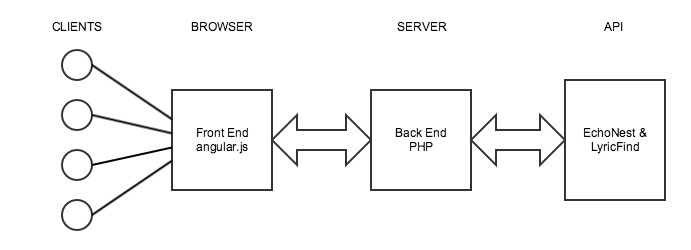
\includegraphics{system_arch.jpg}
\caption{System Architecture}
\end{figure}

This system architecture diagram displays the communication paths of
C-Lyrics. There are three logical entities in our architecture: the
browser, the server, and the external API. The clients exclusively
interact with the front end browser running angular.js. The front end
then makes requests to the server which communicates with the API to
obtain artist data. These data are then communicated back through the
server and displayed on the front end which then communicates with the
clients.

\subsection{2.1 Data Flow Diagram}\label{data-flow-diagram}

\begin{figure}[htbp]
\centering
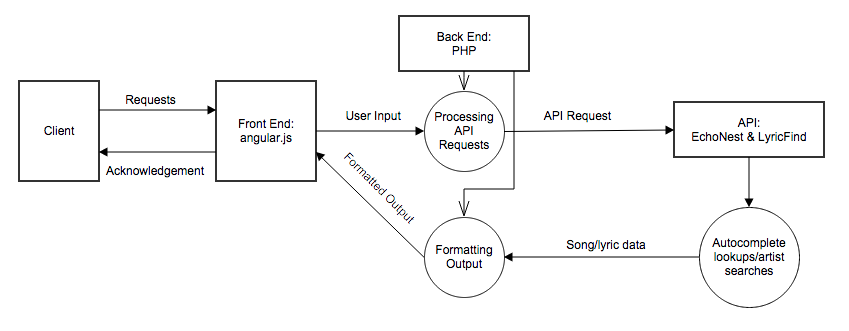
\includegraphics{data_flow.png}
\caption{Data Flow Diagram}
\end{figure}

Above is the data flow diagram for C-Lyrics. Data in the form of
requests are sent to the front end (Browser) as user input. This input
is sent to the server and processed into API requests by the back end
PHP. The input can be of various types (i.e.~artist searches, word
selections, song selections, etc.) and the processed API request goes to
the external API and returns the relevant song/lyric data. This data is
formatted by the backend into the proper form of output (song list, word
cloud, etc.) which is then displayed by the front end browser. The
client then receives the output as acknowledgement.

\section{3 System Design}\label{system-design}

\subsection{3.1 UML Class Diagrams}\label{uml-class-diagrams}

\subsubsection{3.1.1 Server Side Class
Diagram}\label{server-side-class-diagram}

\begin{figure}[htbp]
\centering
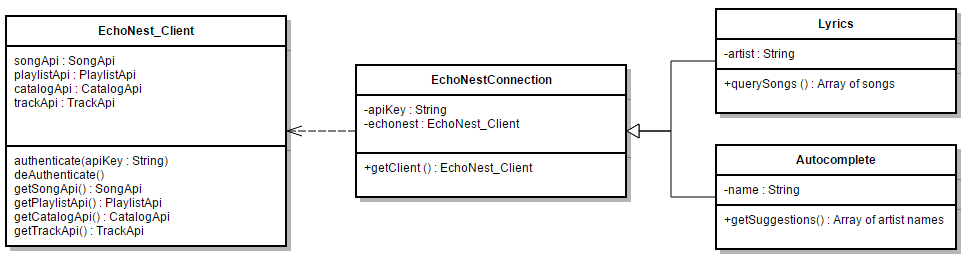
\includegraphics{php_class_design.png}
\caption{Server Side Class Diagram}
\end{figure}

The PHP class diagram illustrates the connection between the
EchoNest\_Client, which is an instance of the EchoNest API, the
EchoNestConnection, along with the subclasses Lyrics and Autocomplete.

The EchoNestConnection class will act as the parent class that has a
single, static connection to the EchoNest API. Both the Lyrics and
Autocomplete will inherit from the EchoNestConnection to query the API.

The class Autocomplete will satisfy the functional requirement of Search
Bar autocompletion. Before the user clicks on the Submit button to
generate the word cloud, the front end will send the current user input
to the getsuggestions php file containing an instance of the
Autocomplete class. The Autocomplete class will then process the input
by using the getSuggestions function, which returns a list of artists
that contain the user input to the getsuggestions page in json format.
The list of artist names will be sent back to the front end to be used
as autocompletion suggestions in the Search Bar.

Once the user clicks on the Submit button, the front end will send the
final artist name to the getlyrics php file containing the instance of
the Lyrics class. The song lyrics for every song by that artist will be
generated by the querySongs function and returned to the getlyrics php
page in json format. The front end will then parse the json data
returned on getlyrics and generate the Word Cloud according to
requirements stated in the SRS document.

\subsubsection{3.1.2 Client Side Class
Diagram}\label{client-side-class-diagram}

\begin{figure}[htbp]
\centering
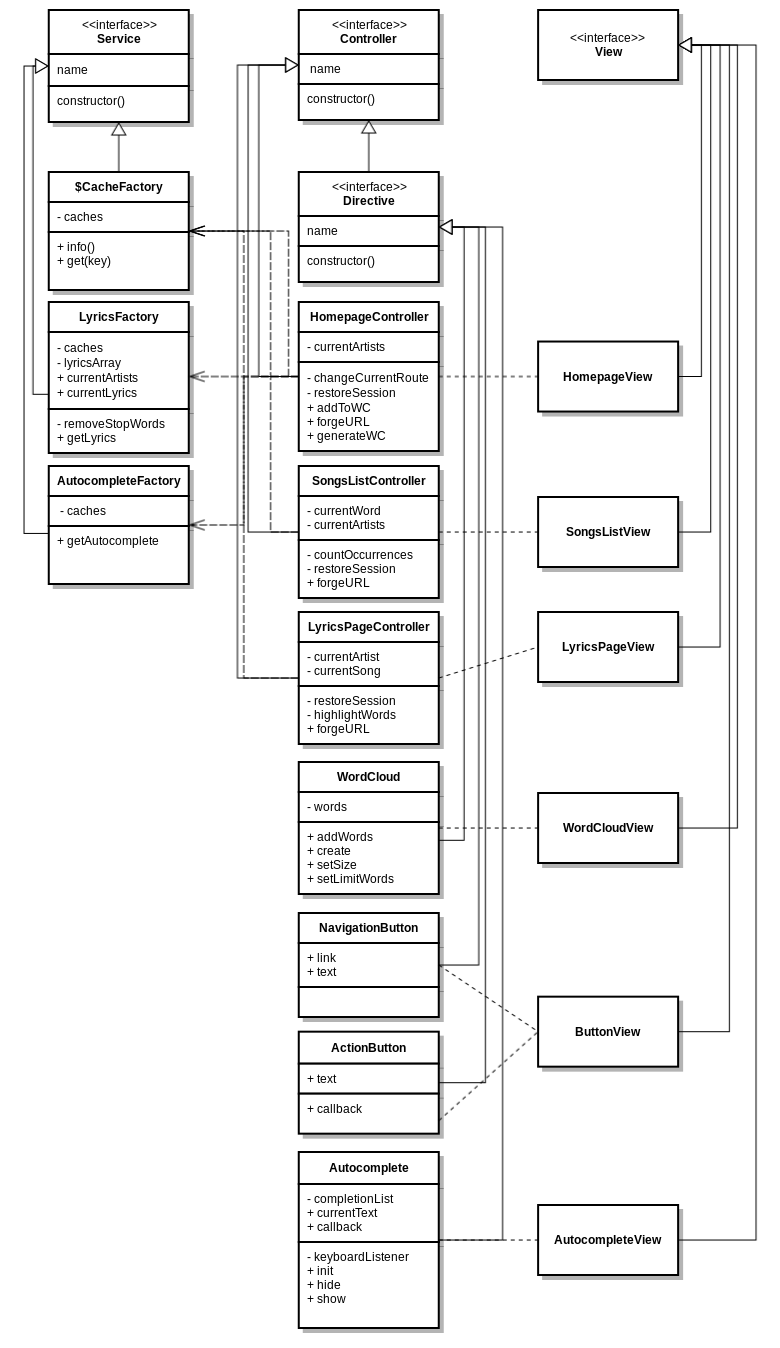
\includegraphics[width=20cm,height=20cm,keepaspectratio]{js_class_design.png}
\caption{Client Side Class Diagram}
\end{figure}

The class diagram exposes the principal relationships between the main
components of the application. The diagram includes some specific
annotations according to the UML standard. The only slight modification
made to the standard occurs with standard dotted lines; the meaning is
that the two connected components are ``semi-codependent'' - they work
separately, but it really makes sense to match them together. Note that
the diagram also includes some components defined by AngularJS, as those
components really help to make sense of the overall design choice.

The layout of the diagram also shows how AngularJS enforces the MVC
pattern. Models are on the left, views on the right and controllers in
the middle. A ``closed'' arrow means inheritance, whereas an open one
involves dependency. Also note that a plus is the sign for a publicly
accessible method or attribute, whereas a minus is private.

An interesting pattern choice is that the HomepageController is the only
component having access to the services and factories. It might appear
differently to the user, for example if he loads a songs page he
previously loaded. The page should still be displayed as it is in the
cache of the browser. However, strictly speaking the user will first be
redirected to the Homepage which will interact with the cache and
present the data to the requested page.

\subsection{3.2 UML Component Diagrams}\label{uml-component-diagrams}

\begin{figure}[htbp]
\centering
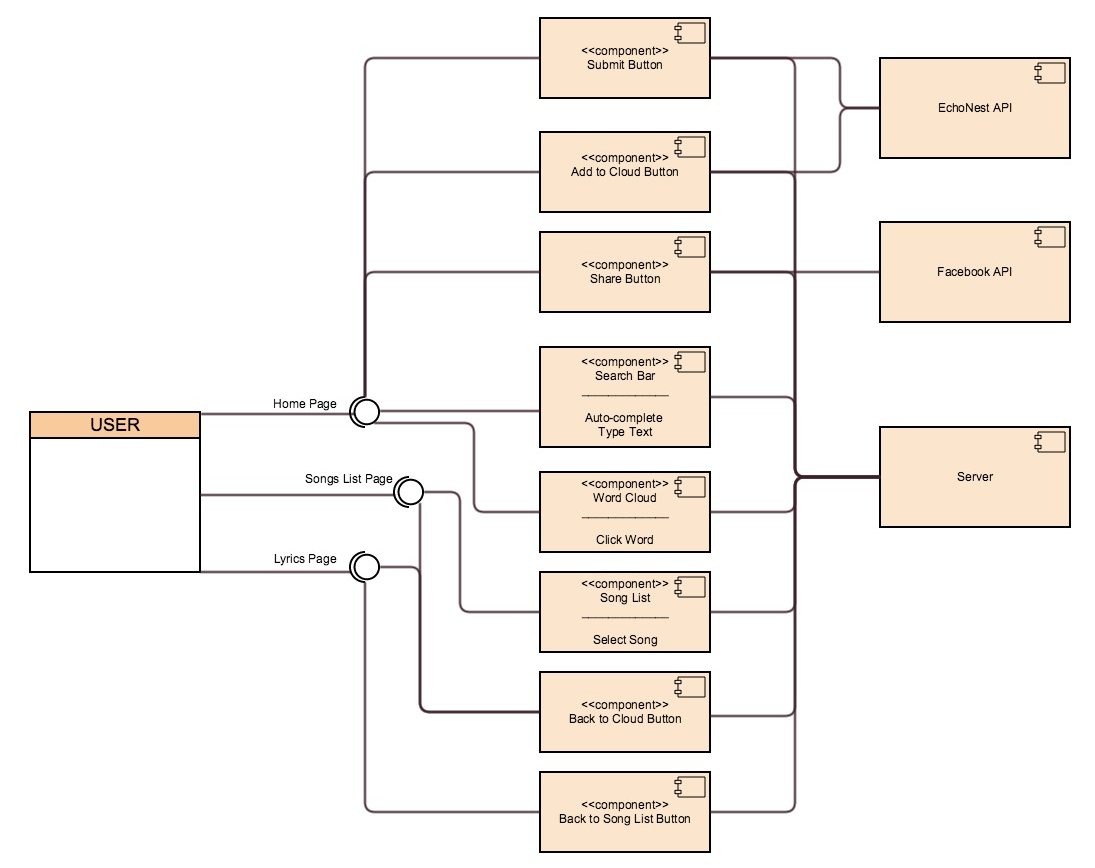
\includegraphics{component_diagram.jpg}
\caption{Component Diagrams}
\end{figure}

The diagram above illustrates the various components in the C-Lyrics
system. These components are key features the user will interact with
during their experience with the C-Lyrics system. It demonstrates the
three interfaces that the user interacts with, such as the Home Page,
the Songs List Page, and the Lyrics Page, as well as which components
each interface has access to. Additionally, the diagram lays out which
components each of the back end communication outlets interacts with.

\subsection{3.3 UML Use Case Diagrams}\label{uml-use-case-diagrams}

\begin{figure}[htbp]
\centering
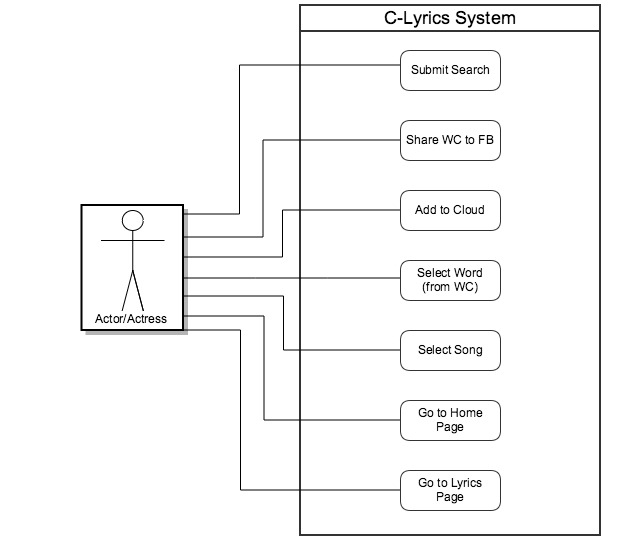
\includegraphics{use_case.jpg}
\caption{Use Case Diagrams}
\end{figure}

In the figure above, a use case diagram is used to represent all
interactions a user, noted as ``Actor/Actress'', will have with the
C-Lyrics system. The interactions a user will have are as follows:

\begin{itemize}
\itemsep1pt\parskip0pt\parsep0pt
\item
  Submit Search: A user will interface with the Home Page and can submit
  their search in the Search Bar to the C-Lyrics system.
\item
  Share Word Cloud (WC) to Facebook (FB): A user will interface with the
  Home Page and can share their generated WC to FB.
\item
  Add to Cloud: A user will type in the Search bar and add to their
  initial search. This will generate a new WC that can be displayed to
  the user.
\item
  Select Word: A user will select any chosen word from the generated WC
  that can lead them to interface with the Songs Page.
\item
  Select Song: On the Songs Page interface, a user can select any song
  from the generated songs list, which will lead them to interface with
  the Lyrics Page.
\item
  Go to Home Page: A user that will interface with either the Songs Page
  or Lyrics Page can be directed back to the Home Page.
\item
  Go to Songs Page: A user that will interface with the Lyrics Page can
  be directed back to the Songs Page.
\end{itemize}

\subsection{3.4 UML State Machine
Diagrams}\label{uml-state-machine-diagrams}

\begin{figure}[htbp]
\centering
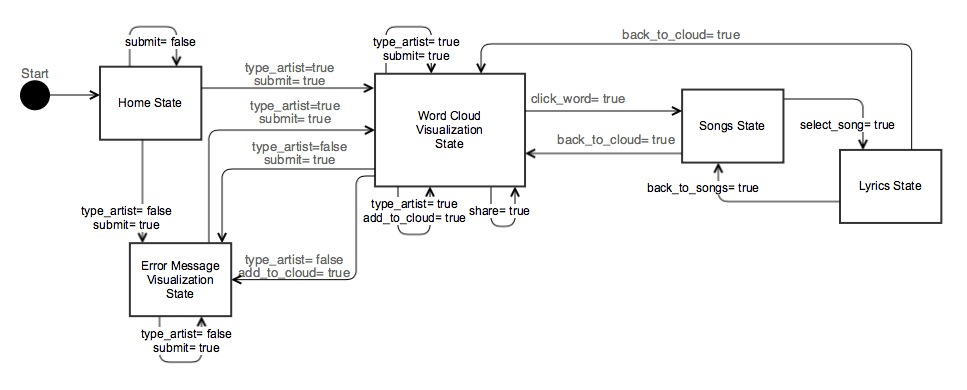
\includegraphics{state_machine.jpg}
\caption{State Machine Diagrams}
\end{figure}

In the state machine diagram above, there are five possible states once
the C-Lyrics system is started. In order to move to another state the
conditions listed must be fulfilled, each condition is represented as a
boolean variable for simplicity. When the user interacts with the
C-Lyrics system, the value of various variables changes depending on the
action performed. Below is an in-depth description of each of the five
states.

\begin{itemize}
\itemsep1pt\parskip0pt\parsep0pt
\item
  Home State

  \begin{itemize}
  \itemsep1pt\parskip0pt\parsep0pt
  \item
    This is the beginning state for the system and represents when the
    user first accesses C-Lyrics. In this state there is no WC
    displayed, only the Search Bar and the Submit Button are on the
    screen. The only actions the user can take from this state are to
    type in the Search Bar and to press the Submit Button.
  \item
    While the Submit Button is not pressed, submit = false and the state
    will not change. If the user presses the Submit Button making submit
    = true then the state will change dependent on the value of the
    type\_artist variable.
  \item
    The type\_artist variable represents the truth value of what the
    user typed into the search bar. If the user entered a valid artist
    name, meaning the artist was found by the API, then type\_artist
    will be true, otherwise it will be false. If type\_artist is false
    then the state will change to Error Message Visualization State, but
    if it is true then the state will change to Word Cloud Visualization
    State.
  \end{itemize}
\item
  Error Message Visualization State

  \begin{itemize}
  \itemsep1pt\parskip0pt\parsep0pt
  \item
    This state represents when the user enters an invalid artist name in
    the Search Bar and presses the Submit Button, causing an error
    message to appear. The only actions the user can take from this
    state are to type in a new artist name to the Search Bar and to
    press the Submit Button.
  \item
    The state will change to Error Message Visualization State every
    time type\_artist = false and either submit = true or add\_to\_cloud
    = true.
  \item
    The the only way to exit this state is when the type\_artist and
    submit variables are both true.
  \end{itemize}
\item
  Word Cloud Visualization State

  \begin{itemize}
  \itemsep1pt\parskip0pt\parsep0pt
  \item
    This state represents when the user is on the Home Page and a WC is
    displayed. From this state the user can perform multiple actions
    some of which will not lead to a state change, as described in the
    bullet points below, and some of which will lead to a state change.
  \item
    If the user types an artist name and both type\_artist and submit
    are true then the user will stay in this state, but a new WC with
    the new artist's information will be displayed. However, if the user
    types an artist name and type\_artist = false but submit = true then
    the state will change to Error Message Visualization State.
  \item
    If the user types an artist name and both type\_artist and
    add\_to\_cloud are true then the user will also stay in this state,
    but the word cloud will be modified to include the information from
    the second artist. However, if the user types an artist name and
    type\_artist = false but add\_to\_cloud = true then the state will
    change to Error Message Visualization State.
  \item
    If the user presses the share button making share = true, then the
    user will stay in this state, but will be able to share the image to
    Facebook via the Facebook API.
  \item
    The state will change to Songs State when the user clicks a word in
    the word cloud making click\_word = true.
  \end{itemize}
\item
  Songs State

  \begin{itemize}
  \itemsep1pt\parskip0pt\parsep0pt
  \item
    This state represents the list of songs that the selected word
    appears in by any given artist. The user can either select a
    specific song title or press the Back to Cloud button from this
    state, both of these actions will lead to a different state.
  \item
    If the user selects a song then select\_song = true and the state
    will change to Lyrics State
  \item
    If the user presses the Back to Cloud Button making back\_to\_cloud
    = true then the state will change to Word Cloud Visualization State.
  \end{itemize}
\item
  Lyrics State

  \begin{itemize}
  \itemsep1pt\parskip0pt\parsep0pt
  \item
    This state represents the lyrics of the song that was selected in
    the Songs Page state. The only actions the user can take from this
    state are pressing the Back to Cloud Button and the Back to Songs
    Button.
  \item
    If the user presses the Back to Songs Button making back\_to\_songs
    = true then the state will change to Songs Page.
  \item
    If the user presses the Back to Cloud Button making back\_to\_cloud
    = true then the state will change to Word Cloud Visualization State.
  \end{itemize}
\end{itemize}

\subsection{3.5 UML Sequence Diagrams}\label{uml-sequence-diagrams}

\begin{figure}[htbp]
\centering
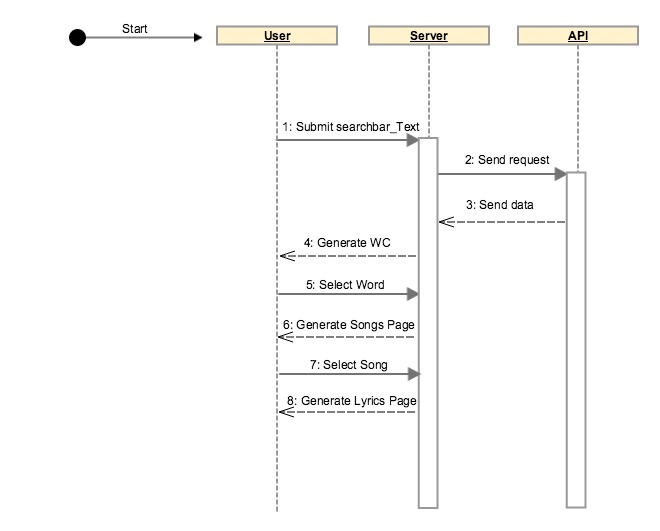
\includegraphics{sequence_diagram.jpg}
\caption{Sequence Diagrams}
\end{figure}

In the figure above, a sequence diagram is used to represent one of the
processes, namely the Select Songs feature, within C-Lyrics. This
sequence diagram shows how the process will interact with the server and
the EchoNest API in order to arrive at the Select Songs feature. Several
terms used in the diagram can be referenced in section 1.4. The diagram
is as follows:

\begin{itemize}
\itemsep1pt\parskip0pt\parsep0pt
\item
  The user will submit their search to the server.
\item
  The server will send a request to the API.
\item
  The API will receive the request based on the information given from
  the user, and send all data on that search to the server.
\item
  The server will then generate a Word Cloud (WC) and display it back to
  the user
\item
  The user can select a word on the WC.
\item
  The server will take in the request from the user and generate the
  second interface, the Songs Page.
\item
  The user can select a song from the Songs Page list.
\item
  The server will take in the request from the user and generate the
  third interface, the Lyrics Page.
\end{itemize}

\section{4 Design Evaluation}\label{design-evaluation}

\subsection{4.1 Validation}\label{validation}

The following list of requirements comes from the Functional
Requirements (FR) section of the SRS. Next to each requirement is a
reference to where in this design document that requirement is
satisfied.

\begin{itemize}
\itemsep1pt\parskip0pt\parsep0pt
\item
  FR1. Web Application-Search Bar: sections 3.1.1 and 3.1.2, front and
  back end search bar functionality
\item
  FR2. Web Application-Word Cloud: sections 3.1.1, 3.1.2 and 3.4 (state
  machine)
\item
  FR3. Web Application-Song List: sections 2.1.1 and 3.4
\item
  FR4. Web Application-Lyrics: sections 3.1.1, 3.1.2, 3.2 and 3.4
\item
  FR5. Access Through Web: sections 2.1 and 2.2
\item
  FR6. Web Application-Share: sections 3.1.1, 3.3, 3.4
\item
  FR7. Web Application-Add to Cloud section 3.1.3
\end{itemize}

\subsection{4.2 Justification of Design
Choices}\label{justification-of-design-choices}

\subsubsection{4.2.1 Data Flow Diagram
Evaluation}\label{data-flow-diagram-evaluation}

The initial level of discourse chosen for the abstraction of our data
flow design is of the application as a whole (step-wise refinement). The
data is viewed as travelling from module to module and from function to
function. Each module encapsulates smaller modules and functionalities
which are hidden from the user of the application. The design exhibits
both strong coupling and cohesivity making it strong in modularity. For
example, the front and back end display communicational cohesion as well
as procedural and sequential cohesion. The front and back end also
display data, control and common coupling as the data passed from the
user is simple text. This data coupling and communicational cohesion is
also present between the front end, back end and API. The backend and
API design is of high quality since the API is essentially a black box
whose functionality is a secret that neither the front end or back end
are aware of, thus reducing coupling between these elements and the API.

\subsubsection{4.2.2 UML Class Diagram
Evaluation}\label{uml-class-diagram-evaluation}

These design principles for the php backend create optimal abstraction
because of the separation of the API client and the classes making the
queries. The Lyrics and Autocomplete php classes each have one purpose
and are broken down to their simplest levels, which only return the type
of requested data in json format. This reduces the complexity of each
class and reduces the number of lines of code, following Object Oriented
Principles of class simplicity. Both classes use communicational
cohesion and external coupling by operating on the same instance of
EchoNest\_Client in EchoNestConnection. In itself, the backend is a
black box for the user. The Lyrics and Autocomplete classes do not rely
on each other, only on the parent class, and can work independently,
reducing the risk of any problems associated with coupling.

By using the AngularJS framework, the design strongly enforces an MVC
pattern. This allows to clearly decouple some parts of the application
in order to gain flexibility and modularity. This schema is underlined
by the different columns of the figure, where the system's
communication, logic and visual interface are separated.

By using directives, the systems allows for reusability of components as
well as a template-directive hierarchy. For example, the ActionButton
class will be used for both the submit button and the add to cloud
button. In addition, the visual template used (ButtonView) is also
shared by the NavigationButton class, which in turns will be used for
both the back to cloud button and the return button.

Finally, this design provides an easy way to extend the application. In
the case where some new functionality should be implemented, the problem
could be approached in two ways. Either the client would like to enhance
the current web pages, in which case few modifications to the
controller, template and a new factory should provide enough flexibility
for the implementation. Another approach would be to add a new web page
to the application which would mean creating a new template and
controller. In both cases, the offered level abstraction by the system
allows to easily implement one's own features in the system. In
addition, the use of existing components is simplified as for each of
them understanding their interface only requires to understand their
public methods. This approach of hiding unnecessary information is also
greatly simplified thanks to the use of AngularJS.

\subsubsection{4.2.3 UML Component Diagram
Evaluation}\label{uml-component-diagram-evaluation}

The component diagram, as seen in section 3.2, is an abstraction of all
of the main parts of the C-Lyrics system and how they interact with the
user through each interface as well as how they interact with the back
end of our system through either the server or chosen APIs. The features
chosen to break into components by following the communicational
cohesion model, features that interact with the same data are coupled
together. Furthermore, the diagram follows the common coupling model
because any component that shares data through a given interface or back
end communication outlet is linked together. These methods of cohesion
and coupling lend themselves to proper information hiding because only
components that need to share data have access to it. There is no
hierarchy in this diagram, but its intra-modular approach is a very
simple way to display the components of C-Lyrics and how they are
connected.

\subsubsection{4.2.4 UML Use Case Diagram
Evaluation}\label{uml-use-case-diagram-evaluation}

The purpose of a class diagram is to create a high level representation
of the interaction a user will have with the C-Lyrics system. The class
diagram, referenced in section 3.3, represents this well by abstracting
all key functions the system offers and allowing the user to visualize
what types of interactions are possible. Hidden information that is not
needed for function understanding is implied by these abstractions.

\subsubsection{4.2.5 UML State Machine Diagram
Evaluation}\label{uml-state-machine-diagram-evaluation}

While runtime complexities make our system difficult to accurately
represent as a finite state machine, the main functions of our system
can be abstracted to fit the finite state machine model as explained in
section 3.4. The modularity of each state is based on logical cohesion,
each state is defined by its functionality within the system as the
whole, and control coupling, the actions performed in one state directly
drive the transition between states. Although the diagram is not laid
out in any specific hierarchy, there are four hierarchical levels in the
state machine. The highest level is the Home State followed by the Word
Cloud Visualization and the Error Message Visualization states, followed
by the Song State and finally the Lyrics State.

\subsubsection{4.2.6 UML Sequence Diagram
Evaluation}\label{uml-sequence-diagram-evaluation}

The sequence diagram that can be found in section 3.5 demonstrates one
of the processes that a user will go through while using C-Lyrics. The
select song functionality was chosen against other functionalities
because this process best portrays the capabilities of the C-Lyrics
system, demonstrating the natural direction of requests and generating
pages. The class diagram also represents modularity, specifically
procedural cohesion that shows the order in which a process is being
done. Multiple types of coupling are also utilized including content
coupling, having certain processes as predecessors for others which can
directly affect a process, and common coupling, in which all data
received from the EchoNest API is shared with the interfaces. Although
the sequence diagram does not have a hierarchical level, it demonstrates
the process flow for the selected features as an intra-modular
approach.. One process follows another and will be completed once the
predecessor has finished the request and displayed the request back to
the person.

\section{5. Appendices}\label{appendices}

\subsection{5.1 Design Process}\label{design-process}

From past experience, the development team continued the practice of
meeting multiple times as a full group in order to discuss the design of
C-lyrics. An object oriented approach was agreed upon and rough sketches
and diagrams were drawn to represent data flow with respect to object
oriented policies. The development team also implemented a top down
design methodology and from the onset of the design process applied this
method to the system architecture design. Given the relatively small
list of functional requirements and low inter modular complexity, the
top down approach is justified.

\subsection{5.2 Meeting Documentation}\label{meeting-documentation}

Based on the Project Management Plan, we followed our consistent current
group process. We agreed to meet as a group through various
communication channels and also established physical meeting times and
locations. At each of our meetings we conducted planning and task
division.

February 17, 2015 Met in New Annenberg room 305 to discuss design
processes and gather information. Also did preliminary task division and
abstract discussion of architecture and diagrams.

\begin{figure}[htbp]
\centering
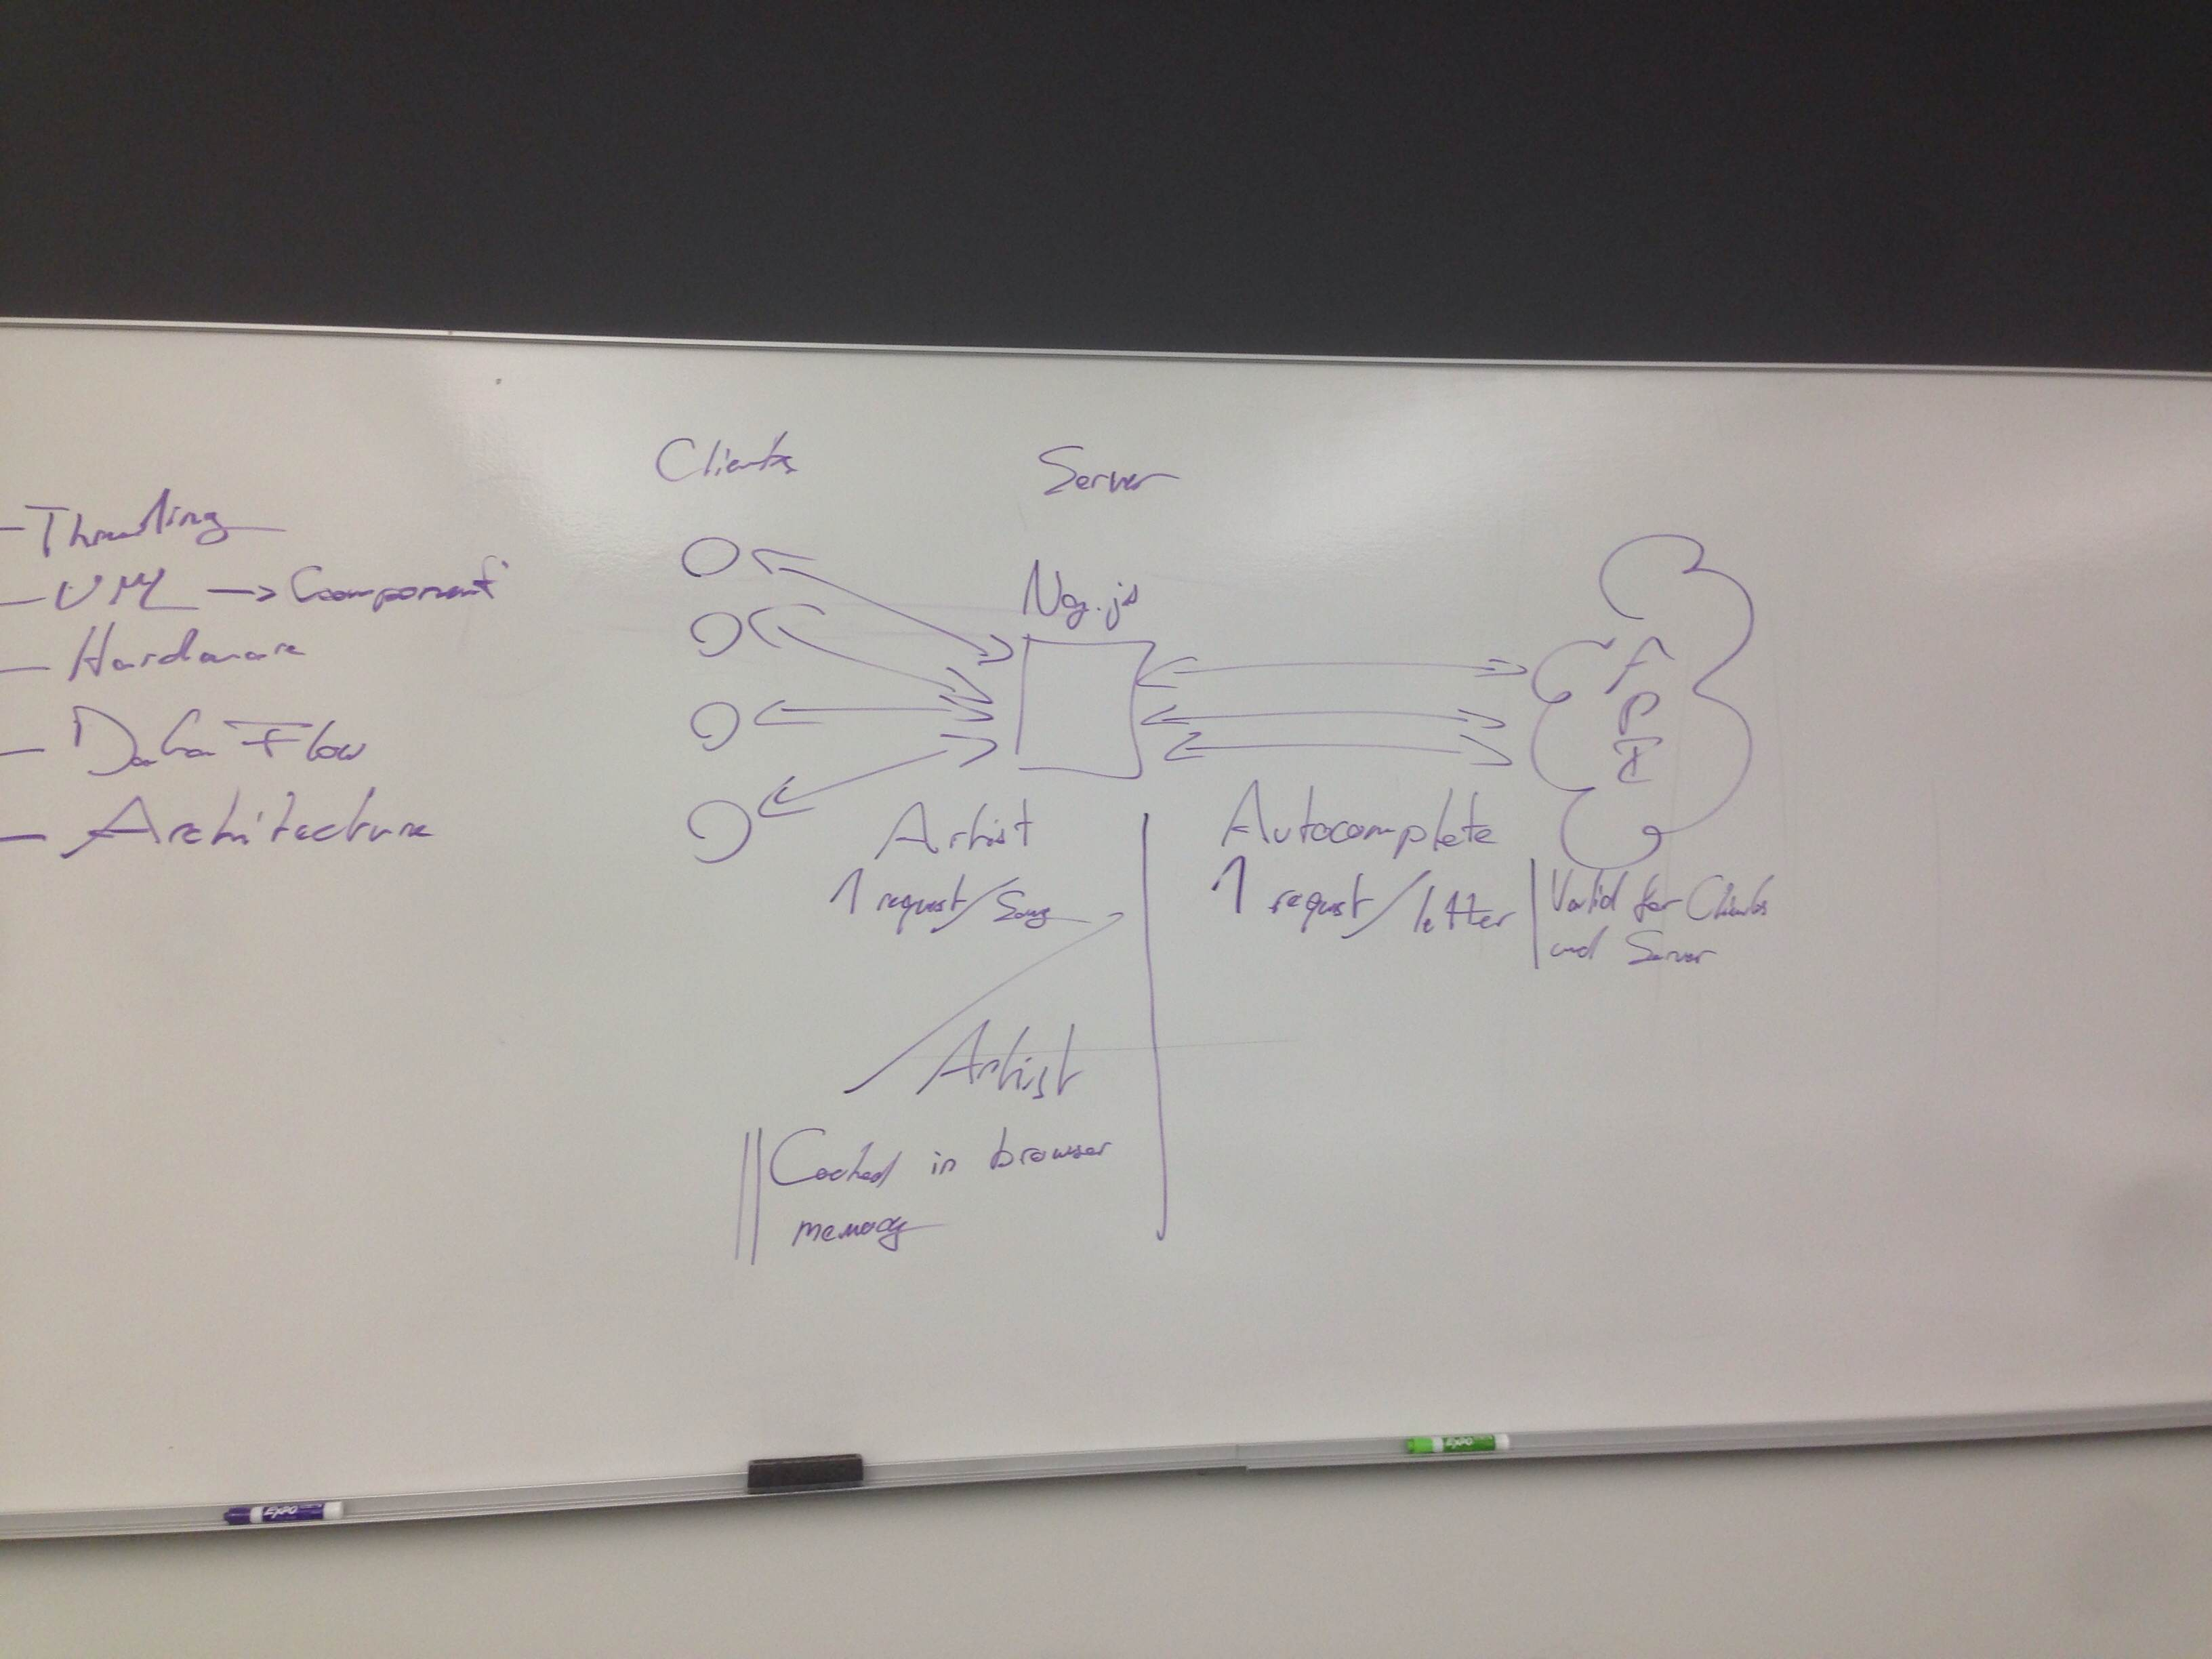
\includegraphics{whiteboard_notes.jpg}
\caption{Whiteboard Notes}
\end{figure}

\subparagraph{Preliminary System Architecture
Design}\label{preliminary-system-architecture-design}

Tentative Staff Allocation:

\begin{itemize}
\itemsep1pt\parskip0pt\parsep0pt
\item
  Mark: PHP related design and class diagram(s) given his past
  experience
\item
  Sebastien: Java Script for front end design, given his past experience
  and familiarity with C-lyrics as lead prototype designer
\item
  Kelsey and Justine: other UML components, given vast experience making
  diagrams and charts
\item
  Milad: unassigned
\end{itemize}

February 18, 2015 Met in Leavey Library with all members of the group.
Exchanged information via gmail.com. Every member contributed
simultaneously to the development of a Google Document holding the rough
draft of this document. Different members proof read the work of others
to check grammar. Tasks were divided as follows:

\begin{itemize}
\itemsep1pt\parskip0pt\parsep0pt
\item
  Justine and Kelsey: System Design and Evaluations
\item
  Mark: PHP Class Diagram and Evaluation
\item
  Sebastien: Angular JS Class Diagram and Evaluation
\item
  Jeff: Architecture and Data Flow Diagrams, Appendix
\item
  Milad: Introduction, Data Flow Diagram Evaluation, Appendix
\end{itemize}

\end{document}
